\documentclass{beamer}
\usetheme{Boadilla}

\title{A case for redundant array of inexpensive disks}
\subtitle{(RAID)}
\author{Siddharth Bhat (20161105)}
\date{\today}

\begin{document}
\begin{frame}
\titlepage
\end{frame}

\begin{frame}
    \begin{itemize}
        \item Moore's law: Transitors in a chip $\times 2$ every 2 years: $\equiv 2^{\frac{\text{Year} - 1964}{2}}$
        \item Bits stored / inch  $\times 10$ every 10 years: $\equiv 10^\frac{{\text{Year} - 1971}}{10}$
        \item SLED (Single Large expensive magnetic disks) cannot keep pace with CPUs!
        \item $Speedup \equiv ??$ Amdahl's law
    \end{itemize}
\end{frame}

\begin{frame}
    \frametitle{Inexpensive Disks}
    \begin{tabular}{lrr}
        & IBM 3380 & Conners CP3100  \\
         Price &\$ 135000 & \textbf{\$1000} \\
         Power/box(Watt) & 6600 W & \textbf{10 W} \\
         IO/sec (max)& \textbf{50 ops/s} & 30 ops/s \\
         IO/sec (typical)& \textbf{30 ops/s} & 20 ops/s\\
         Data capacity (MB) & \textbf{7500 MB} & 100 MB \\
         Time to failure (rated) & 30,000 hours & 30,000 hours \\
         Time to failure (practice) & 100,000 hours & Unk \\
    \end{tabular}

\end{frame}

\begin{frame}
    \frametitle{\textbf{Array} of Inexpensive Disks}
    \begin{tabular}{lrr}
        \tiny
        & IBM 3380 & $135 \times \text{Conners CP3100}$ \\
         Price &\$135000 & \$135000 \\
         Power/box(Watt) & 6600 W & \textbf{1350 W} \\
         IO/sec (max)& 50 ops/s& \textbf{4050 ops/s} \\
         IO/sec (typical)& 30 ops/s & \textbf{2700 ops/s} \\
         Data capacity (MB) & 7500 MB & \textbf{13500 MB} \\
         Time to failure (rated) & \textbf{30,000 hours} & 100 hours  \\
         Time to failure (practice) & \textbf{100,000 hours} & Unk \\
    \end{tabular}


    \begin{alertblock}{The ugly}
    Mean time to failure of any of 135 disks: 30,000 hours / 135 = 100 hours
    \end{alertblock}

\end{frame}

\begin{frame}
    \frametitle{\textbf{Redundant} Array of Inexpensive Disks}
    \begin{itemize}
        \item Extra check disks store redundant information.
        \item Replace failed disk \& replicate from check disk.
    \end{itemize}
\end{frame}

\begin{frame}
    \frametitle{Pleasing side-effects of Redundancy}
    \begin{figure}
    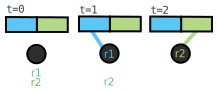
\includegraphics[width=0.5\paperwidth]{seq-reads.pdf}
    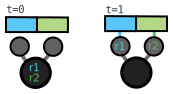
\includegraphics[width=0.5\paperwidth]{par-reads.pdf}
    \end{figure}
    Parallel reads \& writes are enabled to random sections of disk.
\end{frame}

\begin{frame}
    \frametitle{RAID 1: Mirrored Disks}
    \begin{figure}
    \includegraphics[height=0.3\paperwidth]{RAID1.pdf}
    \end{figure}
    \begin{itemize}
        \item All data is duplicated across all disks \pause
        \item Writes are expensive: need to be replicated! \pause
        \item Disk space utilization: \textbf{50\%}.
    \end{itemize}
\end{frame}

\begin{frame}
    \frametitle{RAID 2: Bit level striping + Hamming ECC}
    \begin{figure}
    \includegraphics[height=0.3\paperwidth]{RAID2.pdf}
    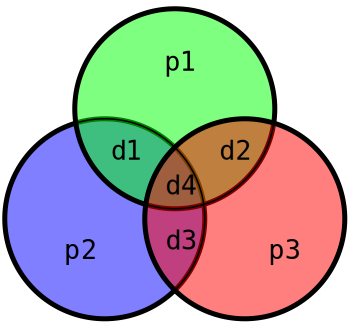
\includegraphics[height=0.3\paperwidth]{hamming.pdf}
    \end{figure}
    \begin{itemize}
        \item Use \textbf{bit-level} striping (consecutive bits $\rightarrow$ different disks).
        \item Use Hamming code \textbf{per bit}. \pause
        \item All disks need to read same bit simultaneously: bitwise error checking. \pause
        \item So, \textbf{Cannot service multiple requests at once}. \pause
        \item Not used anymore.
    \end{itemize}
\end{frame}


\begin{frame}
    \frametitle{RAID 3: Byte level striping + parity ECC}
    \begin{figure}
    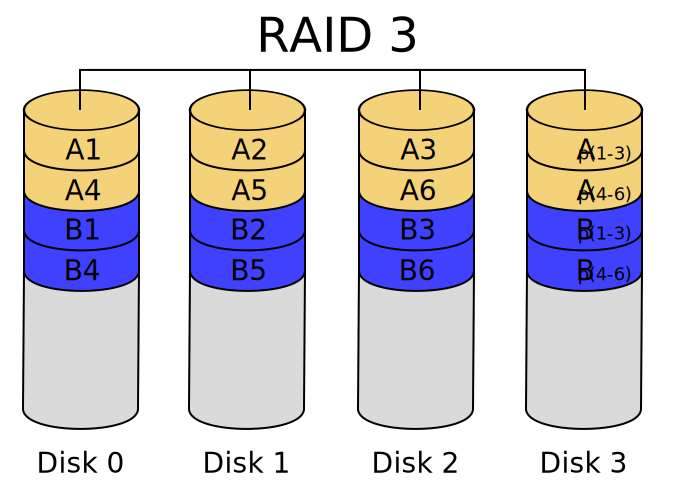
\includegraphics[height=0.3\paperwidth]{RAID3.pdf}
    \end{figure}
    \begin{itemize}
        \item Use \textbf{byte-level} striping (consecutive bytes $\rightarrow$ different disks). \pause
        \item I/O needs \textbf{synchronized spindles}. \pause
        \item parity needs far less storage space. \pause
        \item Rarely used in practice.
    \end{itemize}
\end{frame}


\begin{frame}
    \frametitle{RAID 4: Block level striping + parity ECC}
    \begin{figure}
    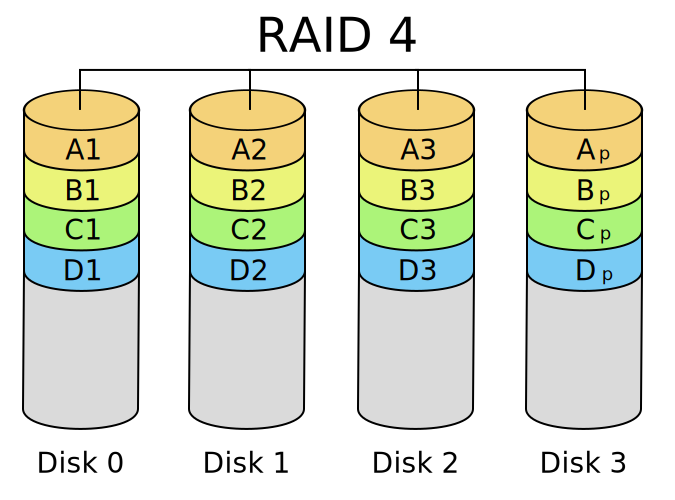
\includegraphics[height=0.3\paperwidth]{RAID4.pdf}
    \end{figure}
    \begin{itemize}
        \item Stripe data per-block (consecutive block $\rightarrow$ different disks). \pause
        \item Block level parity needs far less storage space. \pause
        \item Good random access read times. \pause
        \item Bad write times: All parities in same disk.
    \end{itemize}
\end{frame}

\begin{frame}
    \frametitle{RAID 5: Block level striping + distributed parity ECC}
    \begin{figure}
    \includegraphics[height=0.3\paperwidth]{RAID5.pdf}
    \end{figure}
    \begin{itemize}
        \item Inherits the good from RAID 4. \pause
        \item Good write times: parities distributed across disks.
    \end{itemize}
\end{frame}


\end{document}


